\documentclass[professionalfonts, xcolor={usenames,svgnames,x11names,table}]{beamer}

\usetheme{SBUclass}
\usepackage[charter]{mathdesign}
\usepackage[scaled]{helvet}

\usepackage{mypackages}

\title{\texorpdfstring{Language \& Technology}{Language and Technology}}
\subtitle{Syllabus}
\author{Thomas Graf}
\institute{Stony Brook University\\\texttt{lin120@thomasgraf.net}}
\date{Aug 28, 2016}


\begin{document}
\unnumbered{
\begin{frame}
	\titlepage
\end{frame}
}

\begin{frame}{Organizational Information}
    \begin{center}
        \begin{tabular}{r@{\hspace{2em}}l}
            \textbf{Course}            & Language and Technology\\
            \textbf{Course\#}          & LIN 120\\
            \textbf{Room}              & Humanities 1003\\
            \textbf{Time}              & MW 2:30--3:23\\
            \textbf{Website}           & Blackboard\\[12pt]

            \textbf{Instructor}        & Thomas Graf\\
            \textbf{Email}             & \url{lin120@thomasgraf.net}\\
            \textbf{Office hours}      & M 11:00--12:30 \& 3:30--4:00\\
                                       & W 3:30--4:00\\
                                       & F 11:15--11:45\\
            \textbf{Office}            & SBS N249\\[12pt]

            \textbf{TAs}               & Aniello de Santo \& Al\"{e}na Aks\"{e}nova\\
            \textbf{Undergraduate TAs} & Orel Maimoni \& Suji Yang\\
        \end{tabular}
    \end{center}

    See the Blackboard course page for more details and updates.
\end{frame}


\begin{frame}{Bulletin Description}
    \small

    An introduction to how computers process language and solve language-related tasks. This course discusses the language technologies of our daily life --- spam filtering, machine translation, and many more --- and shows how they work under the hood. The course explores a variety of issues: Why do computers do well in some areas (spell checking) yet fail miserably in others (essay grading)? Will we ever have perfectly fluent AIs as depicted in science fiction? And how will these technological advances impact the role of language in our society? Students will also acquire basic programming skills and write scripts for simple language tasks. No previous training in mathematics or computer science required.    

    \textbf{SBC:} TECH

    3 credits
\end{frame}

\begin{frame}{An Experiment}
    \begin{enumerate}
        \item Open some chat or messaging app on your phone.
        \item Don't type anything.
        \item Instead, click the second word suggestion\\
              (the one in the middle).
        \item Keep doing this.
        \item Did you get a reasonable sentence of English?
    \end{enumerate}

    \visible<2>{
        \begin{quote}
            I am a beautiful person who is the best of luck to you by the way to get the best of luck to you by the way to get the best of luck to you by the way to get the \ldots
        \end{quote}
        }
\end{frame}

\begin{frame}{The Big Take-Home Message}
    \begin{center}
        \begin{tikzpicture}
            \node[draw=Red3,fill=Red3!25,thick,
                  font=\LARGE\bfseries, align=center,
                  inner sep=1em] at (0,0) %
                {Current language technology is mostly\\ smoke and mirrors};
        \end{tikzpicture}
    \end{center}
\end{frame}

\begin{frame}{Questions and Topics}
    \begin{itemize}
        \item How do computers process language?
        \item Why do they succeed in some areas (spell checker, spam filter),\\
            yet fail miserably in others (translation, poetry)?
        \item Will we ever have conversant AIs as depicted in science fiction\\
            (2001, Star Trek, Blade Runner, Her, Ex Machina, System Shock)?
        \item Can computers provide new answers to long-standing questions of linguistics and philology?
        \item How are language communities affected by these new technologies?
    \end{itemize}
\end{frame}

\begin{frame}{Teaching Goals}
    \begin{itemize}
        \item \textbf{Basics of Programming and Computer Science}
            \begin{itemize}
                \item understand the importance of algorithms and data structures
                \item conceptualize linguistic problems in computational terms
                \item basic programming skills in Python
            \end{itemize}
        \pause
        \item \textbf{Cognitive Science}
            \begin{itemize}
                \item familiarity with notions of artificial intelligence
                \item understand how and why humans and computers\\
                    differ in their linguistic abilities
            \end{itemize}
        \pause
        \item \textbf{Digital Humanities and Social Science}
            \begin{itemize}
                \item work with text corpora
                \item use computational tools for humanities\\
                    (stylistic analysis, tracking social developments via corpora)
                \item understand the role of Big Data in computational linguistics
                \item awareness of the dangers of computational linguistics\\
                    (surveillance, language death)
            \end{itemize}
    \end{itemize}
\end{frame}

\begin{frame}{Benchmark}
    By the end of the course, the following scene from \emph{Ex Machina}\\
    should seem rather trivial to you.
    %
    \begin{center} 
         \href{run:exmachina_nlp.mkv}{
            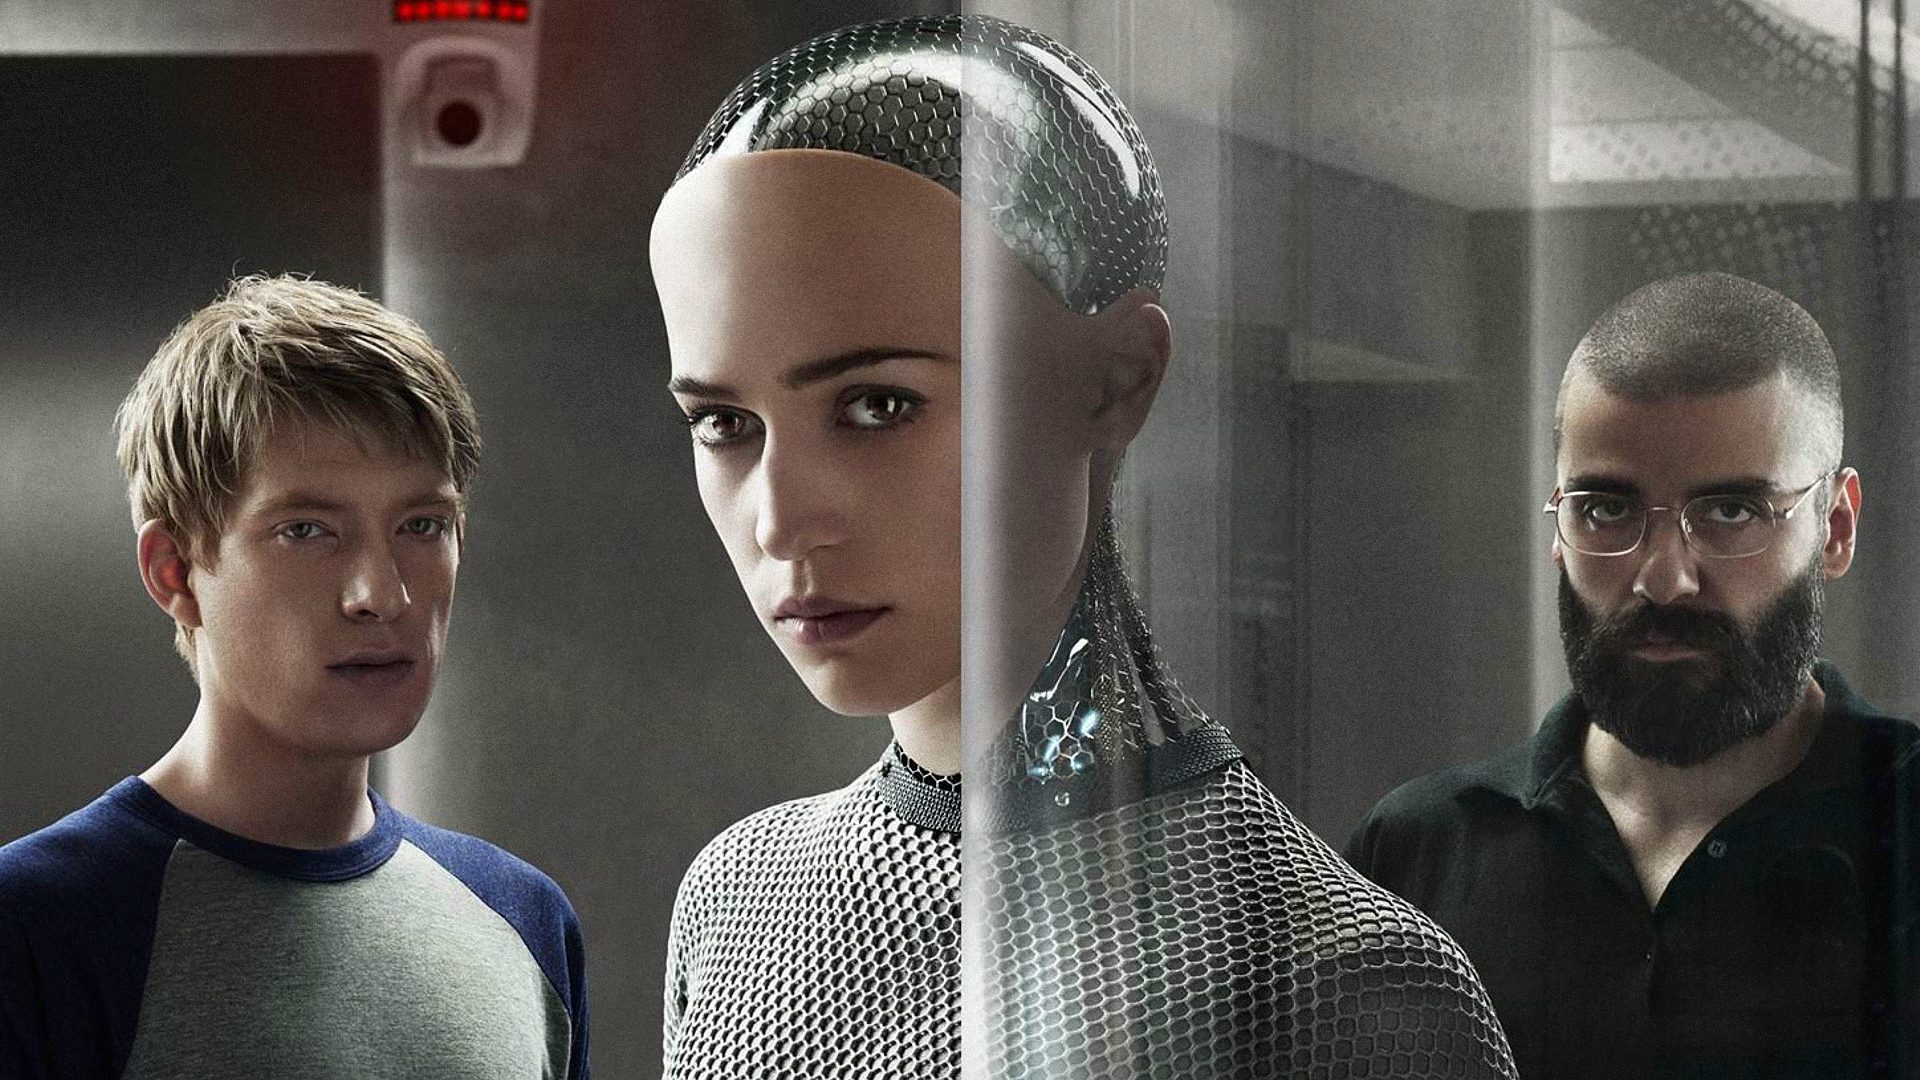
\includegraphics[width=.75\linewidth]{img/exmachina}}
    \end{center}
\end{frame}

\begin{frame}{Prerequisites}
    \begin{itemize}
        \item \textbf{What You Need}
            \begin{itemize}
                \item ability to operate a computer\\
                    (use a web browser, install software, edit text files)
                \item willingness to play around with open-ended problems
            \end{itemize}
        %
        \item \textbf{What You \highlight{WON'T} Need}
            \begin{itemize}
                \item programming experience
                \item math (except for addition, multiplication and fractions)
                \item linguistics (LIN 101 helps a bit, though)
            \end{itemize}
    \end{itemize}
\end{frame}

\begin{frame}{Three Types of Instruction}
    \begin{description}
        \item[Monday] standard lecture on language technology
        \item[Wednesday] programming sessions in Python
        \item[Recitation] recap material with your TAs
    \end{description}

    \begin{center}
        \begin{tabular}{rccc}
                \toprule
                \textbf{Session} & \textbf{Mini-quiz?} & \textbf{Laptop?} & \textbf{Attendance?}\\
                \midrule
                Monday & yes & not recommended & recommended\\
                Wednesday & no & recommended & recommended\\
                Recitation & no & recommended & mandatory\\
                \bottomrule
        \end{tabular}
    \end{center}

    \pause
    \begin{block}{Echo Video Recordings}
        \begin{itemize}
            \item Video recordings of all lectures will be made available online.
            \item But the system is flaky, don't rely on it.
        \end{itemize}
    \end{block}
\end{frame}

\begin{frame}{Grading Components}
    \textbf{Class Participation (20\%)}
        \begin{itemize}
            \item Both in class and \highlight{online}!
            \item \textbf{Examples}:
                \begin{itemize}
                    \item ask questions
                    \item help fellow students
                    \item link to relevant online materials\\
                        $\vdots$
                \end{itemize}
            \item \textbf{Why?} 
                \begin{itemize}
                    \item Encourages you to ask questions.
                    \item Helping others is a great way of learning.
                    \item I want to have some fun, too.
                \end{itemize}
        \end{itemize}
\end{frame}

\begin{frame}{Grading Components [cont.]}
    \textbf{Low-Pressure Exercises (40\%)}
        \begin{itemize}
            \item once per week
            \item programming in \highlight{Python}
            \item assigned on Wednesday at 11:59pm
            \item due the following Wednesday at 11:59pm
            \item only pass-fail grading (0 points VS 1 point)
            \item no late hand-ins (more on that later)
            \item \textbf{Why?}
                \begin{itemize}
                    \item Learning programming is like learning a new language\\
                            $\Rightarrow$ needs constant practice
                    \item Even a little bit of programming experience is incredibly useful.
                \end{itemize}
        \end{itemize}
\end{frame}

\begin{frame}{Grading Components [cont.]}
    \textbf{Mini-Quizzes (40\%)}
        \begin{itemize}
            \item at beginning of Monday lectures
            \item apply techniques discussed in lecture\\
                \subpoint{converting number to binary, listing all character trigrams of a word, $\ldots$}
            \item question templates in online \highlight{quiz pool}
            \item only pass-fail grading (0 points VS 1 point)
            \item missed quiz is an automatic fail (more on that later)
            \item \textbf{Why?}
                \begin{itemize}
                    \item We want you to learn skills and techniques, not definitions.
                    \item Quizzes force you to self-assess how much you're getting out of\\
                        the class.
                \end{itemize}
        \end{itemize}
\end{frame}

\begin{frame}{Dealing with Fails}
    \begin{itemize}
        \item Approximately every 4 weeks you can hand in optional\\
            \highlight{skill assessments}.
            \begin{itemize}
                \item 1 for Python
                \item 1 for Theory
            \end{itemize}
        \item These are take-home exams with multiple assignments.
        \item Each successfully completed assignment converts 1 Fail into a Pass for the respective track (Python\slash Theory).
    \end{itemize}
\end{frame}

\begin{frame}{Example}
    Our example student Stu has the following grades after seven weeks:

    \begin{center}
        \footnotesize
        \begin{tikzpicture}
            \matrix (m) at (0,0) [matrix of nodes, ampersand replacement=\&,
                                  minimum size=1.5em, column sep=.75em, row sep=1em,
                                  row 1/.style = {text=SteelBlue4,font=\bfseries}] {%
                                \& 1 \& 2 \& 3              \& 4 \& [1.5em] \& [1.5em] 5      \& 6 \& 7              \& [1.5em] \\
                \textbf{Quiz}   \& P \& P \& \alt<1>{F}{\alert{P}}  \& P \& $3/4$   \& F              \& F \& P              \& $0/3$ \\
                \textbf{Python} \& P \& P \& \alt<-3>{F}{\alert{P}} \& F \& $1/4$   \& \alt<-4>{F}{\alert{P}} \& P \& \alt<-4>{F}{\alert{P}} \& $2/3$ \\
            };
            %
            \begin{pgfonlayer}{background}
                \node[draw=purple, fill=purple!25, thick] (label) [below=of m-3-8] {Skill assessment};
                \foreach \Column in {6, 10}
                    {
                    \draw[purple, fill=purple!25, thick] (m-2-\Column.north west) rectangle (m-3-\Column.south east);
                    \draw[purple,thick] (label) -| (m-3-\Column);
                    }
            \end{pgfonlayer}
        \end{tikzpicture}
    \end{center}
    %
    \pause
    \begin{enumerate}[<+->]
        \item His first theory assessment converts quiz 3 from F to P.
        \item Quizzes 5 \& 6 remain F because he got 0 points on assessment 2.\\
              Points from other assessments cannot be used!
        \item His first Python assessment converts exercise 3 from F to P.
        \item His second Python assessment converts exercise 5 and 7 to P.
    \end{enumerate}
\end{frame}

\begin{frame}{Soapbox: My Thoughts on Grades}
    \begin{itemize}
        \item Students are caught up in the \highlight{grade bubble}:
            \begin{itemize}
                \item If I get good grades I will get a job.
                \item If I get bad grades I will fail in life.
            \end{itemize}
        \item This is wrong, wrong, wrong, wrong!
        \item In the real world, nobody cares about your GPA.
        \item Don't focus on grades!
        \item Focus on mastering the skills you need to get the job you want.
    \end{itemize}
\end{frame}

\begin{frame}{Soapbox: My Role in This}
    \begin{itemize}
        \item I am the academic equivalent of a \highlight{fitness trainer}.
        \item You're paying thousands of dollars for me to get you into shape,\\ and I've developed a program for you that will do that.
        \item But you are the one who has to move their body.
        \item Bad techniques like cram learning may get you a good grade,\\
              but you're cheating yourself out of true progress.
        \item If you aren't working towards long-term intellectual growth,\\
            you're flushing tons of money down the toilet.
    \end{itemize}
\end{frame}

\begin{frame}{Soapbox: A Rough Cost Calculation}
    \begin{center}
        \begin{tabular}{cccc}
            \visible<1->{
\includegraphics[width=7em]{./img/mugger1}} &
            \visible<2->{
\includegraphics[width=7em]{./img/mugger2}} &
            \visible<3->{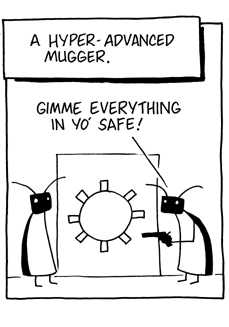
\includegraphics[width=7em]{./img/mugger3}} &
            \visible<4->{
\includegraphics[width=7em]{./img/mugger4}}
        \end{tabular}

        \visible<5>{
        \begin{tabular}{rrr}
            \toprule
            \textbf{Expense} & \textbf{Resident} & \textbf{Non-Resident}\\
            \midrule
            Tuition \& Fees, 12cr & \$5,876.25 & \$14,631.25\\
            Housing \& Meals & $\sim$\$4,500.00 & \$4,500.00\\
            \midrule
            Cost of LIN 120 & \$2594.06 & \$4782.81\\
            Cost per week & \$185.29 & \$341.63\\
            \bottomrule
        \end{tabular}
        }
    \end{center}
\end{frame}

\begin{frame}{Getting Help}
    \begin{itemize}
        \item By default: use discussion forums on Blackboard
        \item Contacting me:
            \begin{itemize}
                \item \url{lin120@thomasgraf.net}
                \item Not using this address means delayed replies!
                \item Reply time usually $<$ 24h
                \item If you plan to come to my office hours, please drop me a line\\
                    the day before.
                    If there's a scheduling conflict, I'll let you know.
                    Radio silence means everything is fine.
            \end{itemize}
        \item For additional instructions, see the \emph{Getting Help} section\\
            on Blackboard.
    \end{itemize}
\end{frame}

\begin{frame}{Some Final Remarks}
    \begin{enumerate}
        \item \textbf{Course Website}
            \begin{itemize}
                \item Familiarize yourself with the course website.
                \item Lots of extra information there.
            \end{itemize}
        \item \textbf{Software Setup}
            \begin{itemize}
                \item We will be using \highlight{Jupyter notebooks}.
                \item See the installation instructions on Blackboard.
                \item More information in Wednesday lecture.
            \end{itemize}
    \end{enumerate}
\end{frame}

\begin{frame}{Supplementary Textbook}
    \begin{columns}
        \column{.65\linewidth}
            \begin{itemize}
                \item Al Sweigart (2015):\\
                      \emph{Automate the Boring Stuff with Python}
                \item online version free
                \item digital versions and hardcopy around \$25
                \item supplementary \href{https://www.youtube.com/playlist?list=PLGoJzB271_7r-iLYuEHEPJ5pSIYxXjJEn}{videos on Youtube}
                \item Only a few parts will be mandatory,\\
                      but it's a good source to consult if something is unclear.
            \end{itemize}

        \column{.35\linewidth}
            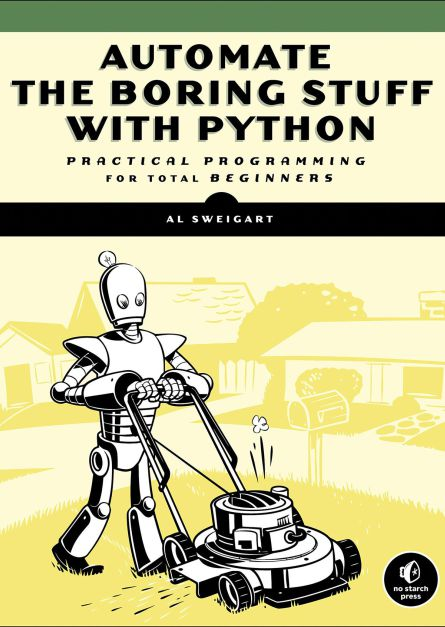
\includegraphics[width=.9\linewidth]{./img/textbook}
    \end{columns}
\end{frame}

\begin{frame}{Your First Homework}
    \begin{enumerate}
        \item Carefully re-read this syllabus.
        \item Read the document \emph{How to Ace This Class} (it's on Blackboard).
        \item There will be a mini-quiz on Wednesday to test your understanding of the course modalities (bring pen and paper!).
    \end{enumerate}

    \textbf{Hint:} Check the quiz pool online for example questions.
\end{frame}


\begin{frame}{Disability Support Services}
    If you have a physical, psychological, medical or learning disability that may impact your course work, please contact Disability Support Services, ECC (Educational Communications Center) Building, Room 128, (631) 632-6748. They will determine with you what accommodations, if any, are necessary and appropriate. All information and documentation is confidential.

    Students who require assistance during emergency evacuation are encouraged to discuss their needs with their professors and Disability Support Services.
    For procedures and information go to the following website:
    \url{http://www.stonybrook.edu/ehs/fire/disabilities}
\end{frame}

\begin{frame}{Academic Integrity}
    Each student must pursue his or her academic goals honestly and be personally accountable for all submitted work. Representing another person's work as your own is always wrong.  Faculty are required to report any suspected instances of academic dishonesty to the Academic Judiciary.  Faculty in the Health Sciences Center (School of Health Technology \& Management, Nursing, Social Welfare, Dental Medicine) and School of Medicine are required to follow their school-specific procedures. For more comprehensive information on academic integrity, including categories of academic dishonesty, please refer to the academic judiciary website at
    \url{http://www.stonybrook.edu/uaa/academicjudiciary/}
\end{frame}

\begin{frame}{Critical Incident Management}
    Stony Brook University expects students to respect the rights, privileges, and property of other people. Faculty are required to report to the Office of Judicial Affairs any disruptive behavior that interrupts their ability to teach, compromises the safety of the learning environment, or inhibits students' ability to learn.  Faculty in the HSC Schools and the School of Medicine are required to follow their school-specific procedures.
\end{frame}

\end{document}
